\documentclass[a4paper]{article}
\usepackage[pdftex]{graphicx}
\usepackage[utf8]{inputenc}
\usepackage{enumerate}
\usepackage{siunitx}
\sisetup{locale=DE} 
\usepackage{icomma}
\usepackage{amssymb}
\usepackage{tikz}
\usepackage{href-ul}
\hypersetup{
	colorlinks=true,
	linkcolor=blue,
	urlcolor=blue}
\usepackage{geometry}
\geometry{a4paper, top=15mm, left=15mm, right=15mm, bottom=15mm,
	headsep=10mm, footskip=12mm}

\begin{document}
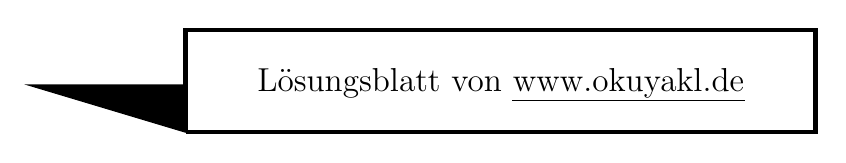
\begin{tikzpicture}(10,3)
	\draw[ultra thick](2,0) --(10,0) -- (10,1.3) --(2,1.3) -- (2,0);
	\draw[fill=black](2,0)-- (0,.6) -- (2,.6) -- (2,0);
	\node at (6,.6) {\large Lösungsblatt von \href{https://www.okuyakl.de}{www.okuyakl.de}};
\end{tikzpicture}
\vspace{0.5 cm}

\noindent{\bf Aufgabe 1. a)}\\
Für die Coulombkraft zwischen zwei geladenen Teilchen gilt:
$$F_C = {1 \over 4 \pi \varepsilon_0}\cdot {Q_1\cdot Q_2 \over r^2}$$
Wir setzen für die Ladungen $Q_1$ und $Q_2$ je eine Elementarladung ein und erhalten:
$$F_C = {1 \over 4 \pi \SI{8,85e12}{\ampere\second\over \volt\meter}}\cdot {(\SI{1,60e-19}{\ampere\second})^2 \over (\SI{5,3e-11}{\meter})^2}=\SI{8,2e-8}{\newton}$$
Einheitencheck:
$$\SI{}{(\ampere\second)^2 \over {\ampere\second \over \volt\meter} \cdot m^2}=\SI{}{\ampere\second \cdot \volt\meter \over \meter^2}= \SI{}{\joule \over \meter} = \SI{}{\newton} $$
\vspace{0.5 cm}

\noindent{\bf Aufgabe 1. b)}\\
Um die Gravitationskraft zu erhalten, wenden wir das Gravitationsgesetz an und setzen die Massen von Proton und Elektron sowie die Gravitationskonstante G ein:  
$$ F_G = {G \cdot m_1 \cdot m_2 \over r^2} = { \SI{6,67e-11}{\meter^3 \kilogram^{-1} \second^{-2}} \cdot\SI{1,67e-27}{\kilogram} \cdot\SI{9,1e-31}{\kilogram} \over (\SI{5,3e-11}{\meter})^2}=\SI{3,6e-47}{\newton}$$
Einheitencheck:
$$\SI{}{{\meter^3 \kilogram^{-1} \second^{-2}} \cdot {{\kilogram^2} \over \meter^2}}= \SI{}{\kilogram \cdot {\meter \over \second^2}} = \SI{}{\newton}$$
Die Gravitationskraft ist also viele Größenordnungen kleiner und damit völlig vernachlässigbar.
\vspace{0.5 cm}

\noindent{\bf Aufgabe 2.}\\
Wir setzen Gravitations- und Coulombkraft gleich und lösen nach der Ladung $Q_2$ auf:
$$
\renewcommand{\arraystretch}{2}
\begin{array}{rcll}
F_G & = & F_C \\
{G \cdot m_1 \cdot m_2 \over r^2} & = & {1 \over 4 \pi \varepsilon_0}\cdot {Q_1\cdot Q_2 \over r^2} & | \cdot r^2 \\
G \cdot m_1 \cdot m_2 & = &  {1 \over 4 \pi \varepsilon_0}\cdot Q_1\cdot Q_2 & |\cdot  4 \pi \varepsilon_0 \\
G \cdot m_1 \cdot m_2 \cdot  4 \pi \varepsilon_0 & = & Q_1\cdot Q_2
&| : Q_1 \\
{G \cdot m_1 \cdot m_2 \cdot  4 \pi \varepsilon_0 \over Q_2} & = & Q_1 \\
Q_1 & = & {\SI{6,67e-11}{\meter^3 \kilogram^{-1} \second^{-2}} \cdot (\SI{1,0e-3}{\kilogram})^2 \cdot  4 \pi \cdot \SI{8,85e-12}{\ampere\second\over \volt\meter} \over\SI{1,0e-13}{\ampere\second}} &=\SI{7,4e-14}{\ampere\second} 
\end{array}
$$
Einheitencheck:
$$\SI{}{{\meter^3 \kilogram^{-1} \second^{-2}} \cdot \kilogram^2 \cdot {\ampere\second\over \volt\meter} \over \ampere\second} = \SI{}{\kilogram \cdot {\meter^2 \over \second^2} \over \volt } = \SI{}{\joule \over \volt} = \SI{}{\volt\cdot \ampere\second \over \volt}  = \SI{}{\ampere\second} = \SI{}{\coulomb} $$
Die Ladung muss nur den sehr kleinen Wert von $\SI{7,4e-14}{\coulomb}$ betragen, also $\SI{0,074}{\pico\coulomb}$, dies entspricht etwa 460000 Elektronen.
\vspace{0.5 cm}

\noindent{\bf Aufgabe 3.}\\
\begin{minipage}{0.6\textwidth}
	Wir berechnen zunächst aus der gegebenen Geometrie den Winkel $\alpha$:
	$$ \sin \alpha = {0,5\cdot d \over l} \Rightarrow \alpha = \sin^{-1} \left( {\SI{0,2}{\meter} \over \SI{1,0}{\meter}} \right)$$
	$$ \alpha = \SI{11,5}{\degree}$$
    Dieser Winkel tritt im Kräfterechteck unterhalb der Kugeln noch jeweils einmal auf. Für die Beträge der Coulomb- und der Gewichtskraft gilt:
    $$ \tan{\alpha} = {F_C \over F_G}$$
    Damit erhalten wir für $F_C$:
    $$F_C = F_G \cdot \tan{\alpha} = \SI{0,05}{\newton} \cdot \tan{\SI{11,5}{\degree}} =
    \SI{0,01}{\newton}$$
\end{minipage}
\hspace{1 cm}
\begin{minipage}{0.4\textwidth}
	\includegraphics[width=5 cm]{pelad240.pdf}
\end{minipage}
\vspace{0.5 cm}

\noindent Nun lösen wir die Formel für die Coulombkraft nach der Ladung auf und erhalten für $Q_1=Q_2=Q$:
$$
\renewcommand{\arraystretch}{2}
\begin{array}{rcll}
F_C  & = & {1 \over 4 \pi \varepsilon_0}\cdot {Q^2 \over d^2} & | \cdot r^2 \cdot  4 \pi \varepsilon_0 \\
F_C \cdot 4 \pi \varepsilon_0 \cdot d^2 & = & Q^2 & | \sqrt{\quad}\\
\sqrt{F_C \cdot 4 \pi \varepsilon_0}\cdot d & = & Q \\
Q & = & \sqrt{\SI{0,01}{\newton}  \cdot 4 \pi \cdot\SI{8,85e-12}{\ampere\second \over \volt\meter}} \cdot \SI{0,4}{\meter} \\
Q & = & \SI{4e-7}{\coulomb} 
\end{array}
$$
Einheitencheck:
$$\sqrt{\SI{}{\newton \cdot {\ampere\second\over \volt\meter}}} \cdot \SI{}{\meter} = \sqrt{\SI{}{{\joule \over \meter} \cdot {\coulomb \over \joule \cdot \coulomb^{-1}\cdot \meter}}} \cdot \SI{}{\meter} = \sqrt{ \SI{}{{\coulomb^2} \over {\meter^2}}} \cdot \SI{}{\meter} = \SI{}{\coulomb}$$ 
Der Betrag der Ladung auf den Kugeln ist $0,4\SI{}{\micro \coulomb}$
\vspace{0.5 cm}

\noindent{\bf Aufgabe 4. a)}\\
Der Betrag der elektrischen Feldstärke ist in einem Punkt mit Abstand $r$ vom Kugelmittelpunkt:
$$ E =  {1 \over 4 \pi \varepsilon_0}\cdot {Q \over r^2} =
  {1 \over 4 \pi \SI{8,85e-12}{\ampere\second\over \volt\meter}}\cdot {\SI{1e-9}{\ampere\second} \over r^2}= \SI{9,0}{\volt\meter} \cdot{1 \over r^2} \qquad (*)$$
\vspace{0.5 cm}

\noindent{\bf Aufgabe 4. b)}\\
Wir setzen für $r$ einmal $R=\SI{4,5}{\centi\meter}$ und einmal $3R=\SI{13,5}{\centi\meter}$ in $(*)$ ein und erhalten:
$$ E_R = {\SI{9}{\volt\meter} \over (\SI{0,045}{\meter})^2}= \SI{4,4}{\kilo\volt\over\meter}$$
$$ E_{3R} =  {\SI{9}{\volt\meter} \over (\SI{0,135}{\meter})^2}= \SI{0,49}{\kilo\volt\over\meter}$$
Also ist die Feldstärke im Bereich $\SI{4,4}{\kilo\volt\over\meter} > E > \SI{0,49}{\kilo\volt\over\meter}$
\vspace{1 cm}

\begin{minipage}{0.5\textwidth}
	\noindent{\bf Aufgabe 4. c)}\\
	\includegraphics[width=8 cm]{kufeld240.pdf}
\end{minipage}
\begin{minipage}{0.45\textwidth}
	\noindent{\bf Aufgabe 4. d)}\\
	Im Inneren der Kugel ist die Feldstärke gleich Null; siehe senkrechte Linie.
	
	\noindent{\bf Aufgabe 4. e)}\\
	Es gilt für die Coulombkraft auf die Probeladung $q$ 
	$$F_C=q \cdot E $$
	Hier ist $q=2\cdot e$ die Ladung des $\alpha$-Teilchens und $E$ die Feldstärke im Abstand von 13,5 cm:
	$$F_C= 2\cdot\SI{1,60e-19}{\coulomb} \cdot \SI{490}{\volt\over\meter}=\SI{1,6e-16}{\newton}$$
	Einheitencheck:
	$$ \SI{}{\coulomb \cdot {\volt\over\meter}} = \SI{}{\coulomb \cdot {\joule \over \coulomb\cdot \meter}} = \SI{}{{\newton \meter \over \meter}} = \SI{}{\newton}$$
\end{minipage}
\vspace{0.5 cm}

\noindent Die Kraft auf den Heliumkern ist von der Kugel weg gerichtet, weil beide Körper positiv geladen sind.
\vspace{0.5 cm}

\noindent{\bf Aufgabe 5. a)}\\
Wir lösen $(*)$ aus Aufgabe 4. a) nach $Q$ auf:
$$
\renewcommand{\arraystretch}{2}
\begin{array}{rcll}
 E_1 & = &  {1 \over 4 \pi \varepsilon_0}\cdot {Q \over d^2} &|\cdot d^2 \cdot 4 \pi \varepsilon_0 \\
 E_1 \cdot d^2 \cdot 4 \pi \varepsilon_0 & = & Q \\
 Q & = & \SI{100}{\volt\over \meter} \cdot (\SI{0,525}{\meter})^2\cdot 4 \pi \cdot\SI{8,85e-12}{\coulomb \over \volt\meter} &= \SI{3,1e-9}{\coulomb}
\end{array}
$$
Einheitencheck:
$$ \SI{}{{\volt\over \meter} \cdot \meter^2 \cdot {\coulomb \over \volt\meter}} = \SI{}{\coulomb}$$
\vspace{0.5 cm}

\noindent{\bf Aufgabe 5. b)}\\
Der Radius des geladenen Ballons spielt keine Rolle für die Feldstärke außerhalb des Ballons. Die Feldstärke im Abstand $d>r_2$ verhält sich so, als ob die gesamte Ladung im Ballonmittelpunkt vereinigt wäre.
\vspace{0.5 cm}

\noindent{\bf Aufgabe 6.}\\

\begin{minipage}{0.3\textwidth}
Für den Abstand $a$ des feldfreien Punktes $P$ von der Ladung $Q_2$ gilt:
$$ a= d-s \quad (**)$$
\end{minipage}
\begin{minipage}{0.65\textwidth}
	\includegraphics[width=10 cm]{fefrei240.pdf}
\end{minipage}
\vspace{0.5 cm}

\noindent Wir verwenden wieder $(*)$, diesmal rechts und links, denn im feldfreien Punkt heben sich beide Feldstärken auf; sie sind hier betragsmäßig gleich und entgegen gerichtet:
$$
\renewcommand{\arraystretch}{2}
\begin{array}{rcll}
E_1 & = & E_2 \\
 {1 \over 4 \pi \varepsilon_0}\cdot {Q_1 \over s^2} & = &  {1 \over 4 \pi \varepsilon_0}\cdot {Q_2 \over a^2} &| \cdot  4 \pi \varepsilon_0 \\
{ Q_1 \over s^2} & = &  {Q_2 \over a^2} & | : Q_1 \cdot a^2 \\
{ a^2 \over s^2} & = &  {Q_2 \over Q_1} & | \sqrt{\quad} \\
{ a \over s} & = & \sqrt{Q_2 \over Q_1} &| (**)\\
{ d-s \over s} & = & \sqrt{Q_2 \over Q_1} \\
{d \over s}-1 & = & \sqrt{Q_2 \over Q_1} &|+1 \quad |\cdot s\\
 d & = & s \cdot \left( \sqrt{Q_2 \over Q_1}+1 \right)\\
 d & = & \SI{0,1}{\meter} \cdot \left( \sqrt{\SI{5,5}{\nano\coulomb} \over \SI{8,5}{\nano\coulomb}}+1 \right) &= 
 \SI{0,18}{\meter}
\end{array}
$$
Der Abstand beider Punktladungen beträgt 18 cm.

\begin{center}
	\includegraphics[width=7 cm]{../../viecher/endcomic.pdf}
	
	Hier geht es zurück zum \href{https://www.okuyakl.de/phys/p11coulL240/aa240.pdf}{Aufgabenblatt}
\end{center}

\end{document}